\begin{frame}[fragile]
  \frametitle{Starting from analogs}
  \begin{columns}[T]
    \begin{column}{0.5\linewidth}
      \begin{center}
        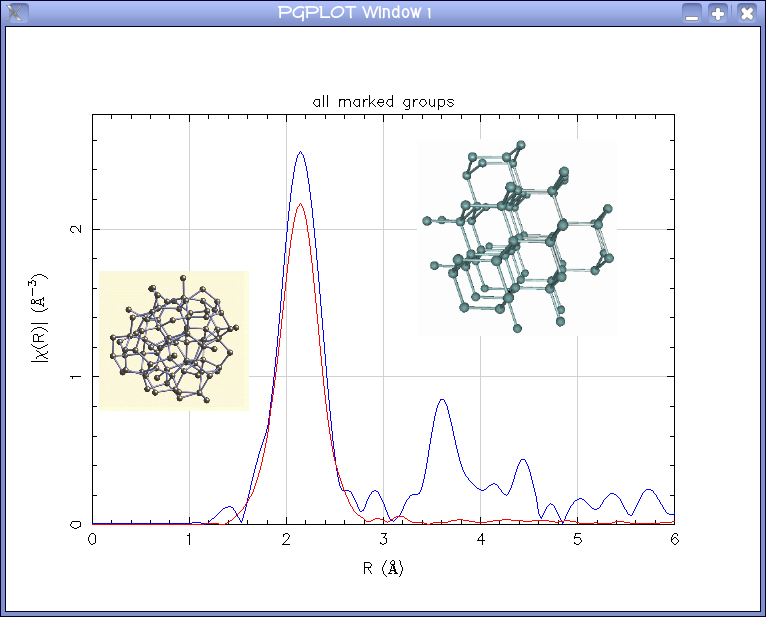
\includegraphics[width=0.9\linewidth]{images/ge_chir_bns}
      \end{center}

      \bigskip

      Use the \texttt{`feff0001.dat'} file from the Ge
      crystal \textsc{feff} calculation

    \end{column}
    \begin{column}{0.5\linewidth}
      \begin{block}{}
        \begin{alltt}
          \tiny
 {\color{Green4}title germanium diamond structure}
 {\color{Brown4}space} f d 3 m
 {\color{Brown4}rmax}=6.0   {\color{Brown4}a}=5.658
 {\color{Brown4}atoms}
 {\color{Blue4}! At.type   x     y     z      tag}
    Ge      1/8   1/8   1/8
         \end{alltt}
       \end{block}

       \begin{center}
         \scriptsize
         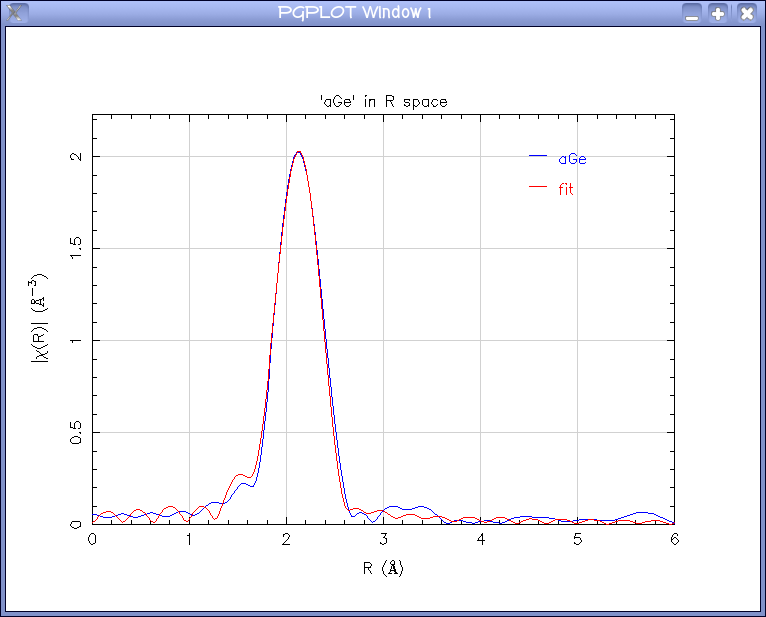
\includegraphics[width=0.85\linewidth]{images/ge_fit}

         \medskip

         \begin{tabular}{lcc}
           & crystal & amorphous \\
           \hline
           N & 4 & 4.0(8) \\
           $R_1$ (\AA) & 2.441(3) & 2.451(11) \\
           $\sigma^2$ (\AA$^2$) & 0.00419(55) & 0.00528(155) \\
         \end{tabular}
       \end{center}
    \end{column}
  \end{columns}
  \begin{textblock*}{0.5\linewidth}(0pt,19\TPVertModule) \tiny
    Crystalline data is from the 
    \href{http://www.nsls.bnl.gov/beamlines/x18b/data.htm}
    {\color{Purple4}NSLS X18 standards database}.
    Amorphous data courteously provided by Dale Brewe and Joe Woicik.
  \end{textblock*}
\end{frame}

\begin{frame}[fragile]
  \frametitle{Close is usually good enough}
  \begin{columns}[T]
    \begin{column}{0.5\linewidth}
      Solid solution of AgBr$_{0.5}$Cl$_{0.5}$ at 20\,K

      \bigskip

      The first shell contains both Br and Cl scatterers.  We use the
      known crystal structure for AgBr to compute the Ag--Br path.
      \begin{block}{}
        \begin{alltt}
          \tiny
 {\color{Green4}title rocksalt silver bromide at room temperature}
 {\color{Brown4}space} F M -3 M
 {\color{Brown4}rmax}=6   {\color{Brown4}a}=5.7745
 {\color{Brown4}core}=Ag
 {\color{Brown4}atoms}
 {\color{Blue4}! At.type   x     y     z      tag}
    Ag      0.0   0.0   0.0
    Br      1/2   1/2   1/2
         \end{alltt}
       \end{block}
       We simply replace Br with Cl and run \textsc{atoms} and
       \textsc{feff} again.
    \end{column}
    %%
    \begin{column}{0.5\linewidth}
      \begin{center}
        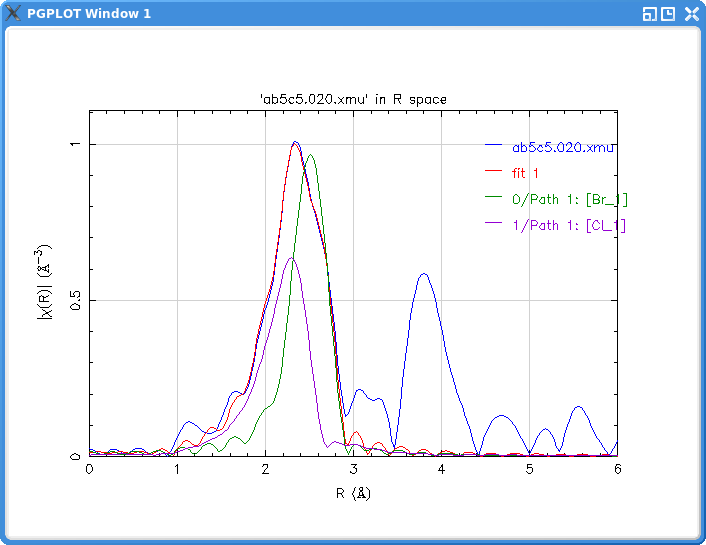
\includegraphics[width=0.9\linewidth]{images/abcfit}

        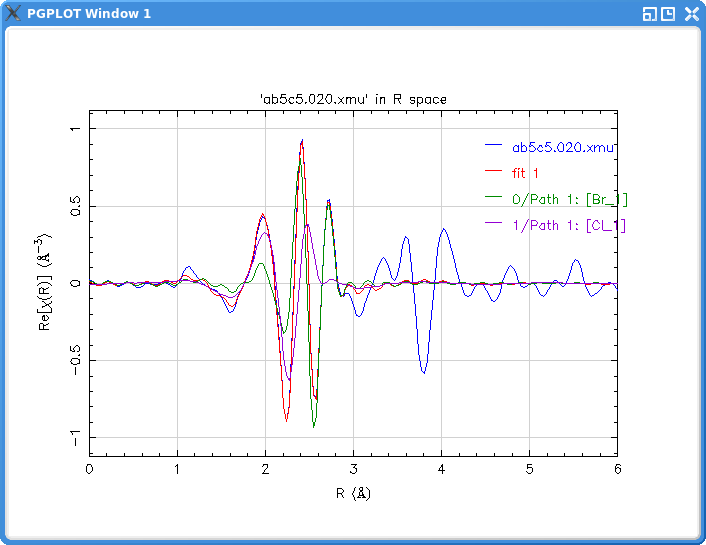
\includegraphics[width=0.9\linewidth]{images/abcfit_re}
      \end{center}

    \end{column}
  \end{columns}

  \medskip

  \begin{center}
    %%\scriptsize{
    $\Delta R_\mathrm{Br}=-0.032(4)\mathrm{\AA}$ \qquad
    {\color{Red3}$\Delta R_\mathrm{Cl}=-0.105(12)\mathrm{\AA}$}
    %%$\sigma^2_\mathrm{Br}=0.00499(41)\mathrm{\AA}^2$,
    %%$\sigma^2_\mathrm{Cl}=0.00719(165)\mathrm{\AA}^2$,
    %%}
  \end{center}
\end{frame}

\begin{frame}
  \frametitle{Pick and choose}
  \begin{columns}
    \begin{column}{0.5\linewidth}
      The data are uranyl acetate mixed with a \textit{B. Subtilis}
      culture and brought to equilibrium at $\mathrm{pH}\sim8$.

      \begin{center}
        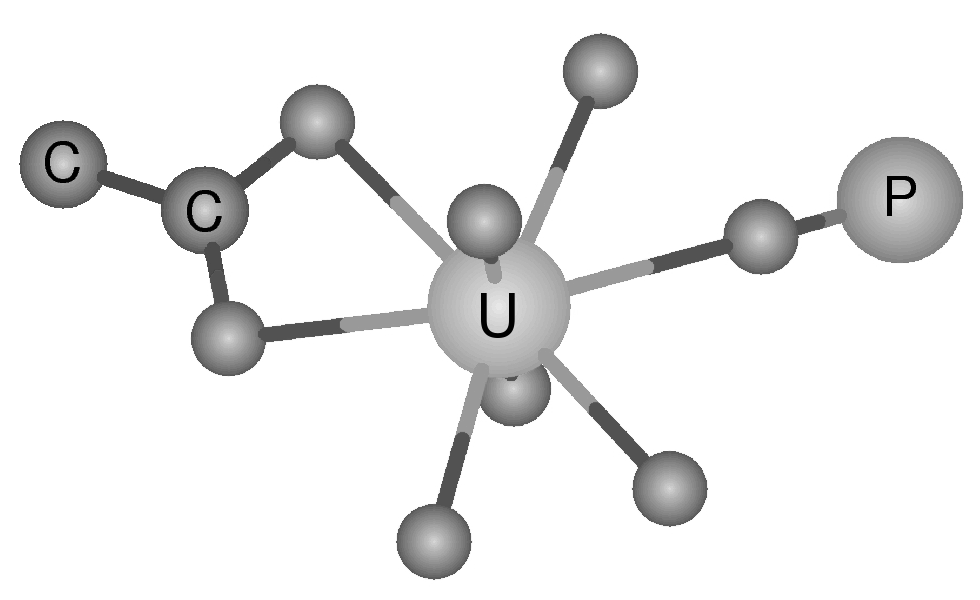
\includegraphics[width=3cm]{images/UPC_bw}
      \end{center}
    \end{column}
    %%%
    \begin{column}{0.5\linewidth}
      \centering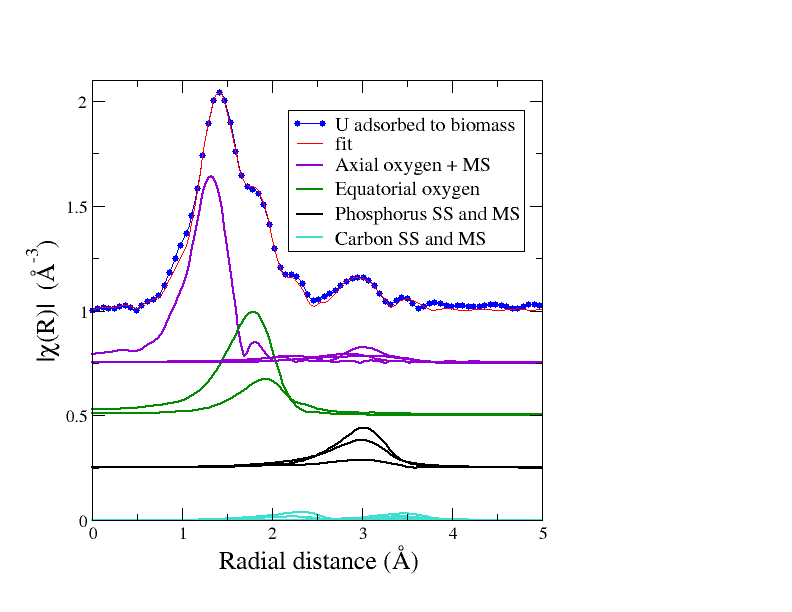
\includegraphics[width=\linewidth]{images/ubs}
    \end{column}
  \end{columns}
  \begin{description}
  \item[triuranyl diphoshate tetrahydrate] This mineral provides paths
    for axial and equatorial O of the appropriate lengths as well as
    SS and MS to the monodentate P
  \item[Rutherfordine, UO$_2$CO$_3$] This mineral provides paths for
    SS and MS involving the bidentate C
  \end{description}
  \begin{textblock*}{0.5\linewidth}(0pt,20\TPVertModule) \tiny S.D.\
    Kelly \textit{et al}., Geochimica et Cosmochimica Acta,
    \textbf{66}:22, pp.\ 3855–-3871, 2002
  \end{textblock*}



\end{frame}

%%% Local Variables:
%%% mode: latex
%%% TeX-master: "pimst2"
%%% End:
